\documentclass{standalone}

\usepackage[OT1]{fontenc}
\renewcommand*\familydefault{\sfdefault}
\usepackage{helvet,sfmath}
\usepackage{siunitx}

\usepackage{tikz}
\usetikzlibrary{arrows,calc,patterns}
\usepackage{tikz,tkz-euclide}

\definecolor{BlueDefault}{rgb}{0.2,0.2,0.7}

\begin{document}

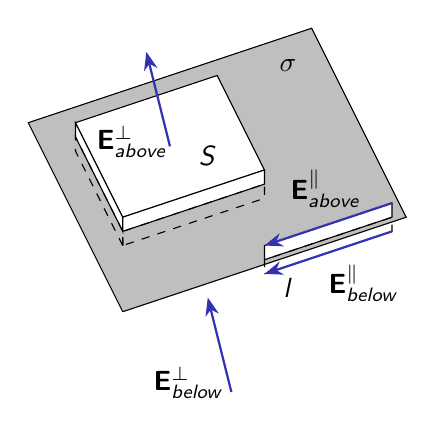
\begin{tikzpicture}[scale=0.6]
            %% Background and boundary
            \draw[fill = lightgray] (2,0) to (0,4) to (6,6) to (8,2) to (2,0);
            \draw (5.5,5.2) node{\( \sigma \)};
            %%flux
            \draw[fill = white] (2,2) to (1,4) to (4,5) to (5,3) to (2,2);
            \draw[fill = white] (2,2) to (1,4) to (1,3.7) to (2,1.7) to (2,2);
            \draw[fill = white] (2,2) to (2,1.7) to (5,2.7) to (5,3) to (2,2);
            \draw[dashed] (2,1.4) to (1,3.4) to (1,3.7) to (2,1.7) to (2,1.4);
            \draw[dashed] (2,1.4) to (2,1.7) to (5,2.7) to (5,2.4) to (2,1.4);
            \draw (3.8,3.3) node{\(S\)};
            %%Circulation
            \draw[fill = white] (5,1.1) to (7.7,2) to (7.7,2.3) to (5,1.4) to (5,1.1);
            \draw[dashed] (5,0.8) to (7.7,1.7) to (7.7,2) to (5,1.1) to (5,0.8);
            \draw (5.5,0.5) node{\(l\)};
            %% Electric field
            \draw[BlueDefault, thick, -Stealth] (3,3.5) to (2.5,5.5);
            \draw[BlueDefault, thick, -Stealth] (4.3,-1.7) to (3.8,0.3);
            \draw 
            (2.2,3.6) node{\( \mathbf{E}_{above}^{\perp} \)}
            (3.4,-1.5) node{\( \mathbf{E}_{below}^{\perp} \)}
            ;
            \draw[BlueDefault, thick, -Stealth] (7.7,1.7) to (5,0.8);
            \draw[BlueDefault, thick, -Stealth] (7.7,2.3) to (5,1.4);
            \draw
            (6.3,2.6) node{\( \mathbf{E}_{above}^{\parallel} \)}
            (7.1,0.6) node{\( \mathbf{E}_{below}^{\parallel} \)}
            ;
            % \draw[-Stealth] (4,-0.5) to (2.5,5.5);
            % \draw[-Stealth] (4.5,-2.5) to (4,-0.5);
\end{tikzpicture}

\end{document}